% CREATED BY DAVID FRISK, 2015
\chapter{Methods}



Lorem ipsum dolor sit amet, consectetur adipisicing elit, sed do eiusmod tempor incididunt ut labore et dolore magna aliqua. Ut enim ad minim veniam, quis nostrud exercitation ullamco laboris nisi ut aliquip ex ea commodo consequat. Duis aute irure dolor in reprehenderit in voluptate velit esse cillum dolore eu fugiat nulla pariatur. Excepteur sint occaecat cupidatat non proident, sunt in culpa qui officia deserunt mollit anim id est laborum.


\section{Geodesic generation}

There are different ways to find or generate geodesic on a surface. In this chapter two possible ways will be described. The two different approaches differs in the sense of its initial condition. Either you can generate the geodesics in a form finding process or you can start from an already defined surface.

\subsection{Dynamic relaxation approach}

It is possible to


'
\begin{figure}[H]
\centering
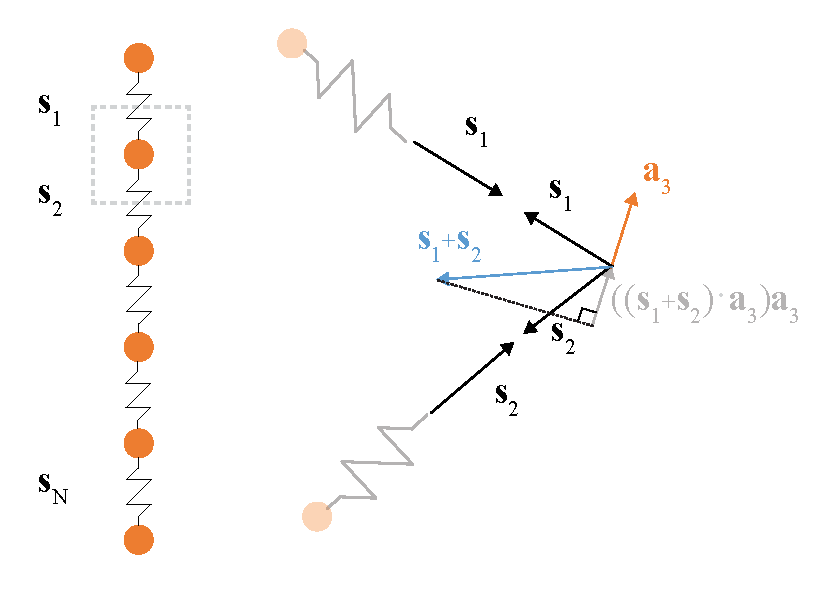
\includegraphics[width = 0.7\linewidth ]{figure/Method/GeodesicDyn.pdf}
\caption{http://web.mit.edu/hyperbook/Patrikalakis-Maekawa-Cho/node29.html}
\end{figure}

\subsection{Dynamic relaxation approach}
